%% file: example.tex = LaTeX + BibTex example for article-like report
%% init: sometime 1993 for my practical "Stellar Spectra A"
%% last: Jan 17 2020  Rob Rutten  Deil
%% site: http://www.staff.science.uu.nl/~rutte101/rrweb/rjr-edu/manuals/student-report/

%% First read ``latex-bibtex-simple-manual'' at
%% http://www.staff.science.uu.nl/~rutte101/Report_recipe.html

%% Then run this file to see what it does:
%%    latex example     bibtex example     latex example     latex example
%% inspect with xdvi example &, or pdflatex into example.pdf for inspection.

%% Take out my content to make a template for your report.

%%%%%%%%%%%%%%%%%%%%%%%%%%%%%%%%%%%%%%%%%%%%%%%%%%%%%%%%%%%%%%%%%%%%%%%%%%%%
\documentclass{aa-note}    %% Astronomy & Astrophysics style class aa.cls v8.2

%% load latex packages
\usepackage{graphicx,url,twoopt,natbib}
\usepackage[varg]{txfonts}           %% old-fashioned A&A font choice
\usepackage{hyperref}                %% for pdflatex
%%\usepackage[breaklinks]{hyperref}  %% for latex+dvips, not for pdflatex
%%\usepackage{breakurl}              %% for latex+dvips, not for pdflatex

%% define link colors
\hypersetup{
  colorlinks=true,   %% links colored instead of frames
  urlcolor=blue,     %% external hyperlinks
  linkcolor=blue     %% internal latex links (eg Fig)
}

\bibpunct{(}{)}{;}{a}{}{,}    %% natbib cite format used by A&A and ApJ
\pagestyle{plain}             %% undo the fancy A&A pagestyle
\let\footnotesize\tiny        %% keep this to 1 page (aa.cls sets \small)

%% Add commands to add a note or link to a reference
\makeatletter
\newcommand{\bibnote}[2]{\global\@namedef{#1note}{#2}}
\newcommand{\biblink}[2]{\global\@namedef{#1link}{#2}}
\makeatother

%% Commands to make citations ADS clickers and to add such also to refs.
%% The twoopt definition permits parameters as in natbib (which I never use).
%% The stonyslink solves a stop problem when using latex instead of pdflatex.
%% May 20 2019: switch to "new" ADS (classic in EDP/A&A readme still work)
\makeatletter
  \protected\def\stonyslink{%
     \def\hyper@linkstart##1##2{}\let\hyper@linkend\@empty}
  \newcommandtwoopt{\citeads}[3][][]{%
   \href{http://ui.adsabs.harvard.edu/abs/#3/abstract}%
        {\stonyslink \citealp[#1][#2]{#3}}%   %% Rutten, 2000
   \biblink{#3}{\href{http://ui.adsabs.harvard.edu/abs/#3/abstract}{ADS}}}
 \newcommandtwoopt{\citepads}[3][][]{%
   \href{http://ui.adsabs.harvard.edu/abs/#3/abstract}%
        {\stonyslink \citep[#1][#2]{#3}}%     %% (Rutten 2000)
   \biblink{#3}{\href{http://ui.adsabs.harvard.edu/abs/#3/abstract}{ADS}}}
 \newcommandtwoopt{\citetads}[3][][]{%
   \href{http://ui.adsabs.harvard.edu/abs/#3/abstract}%
        {\stonyslink \citet[#1][#2]{#3}}%     %% Rutten (2000)
  \biblink{#3}{\href{http://ui.adsabs.harvard.edu/abs/#3/abstract}{ADS}}}
 \newcommandtwoopt{\citeyearads}[3][][]{%
   \href{http://ui.adsabs.harvard.edu/abs/#3/abstract}%
        {\stonyslink \citeyear[#1][#2]{#3}}%  %% 2000
   \biblink{#3}{\href{http://ui.adsabs.harvard.edu/abs/#3/abstract}{ADS}}}
\makeatother

%% ADS specific page opener = {bibcode}{pdf page number}{link text}.
%% ADS promised that the "classic" link below keeps working in "new" ADS;
%% I use it because it opens ADS bibcode pdf's and ADS arXiv altcode pdf's
%% whereas "new" ADS needs separate commands (to PUB_PDF and EPRINT_PDF)
\def\linkadspage#1#2#3{\href{http://adsabs.harvard.edu/cgi-bin/nph-data_query?bibcode=#1\&link_type=ARTICLE\&db_key=AST\#page=#2}{#3}}

%% Spectral species
\def\HI{\ion{H}{I}}            %% A&A; for aastex use \def\HI{\ion{H}{1}}
\def\MgI{\ion{Mg}{I}}          %% A&A; for aastex use \def\MgI{\ion{Mg}{1}}
\def\MgII{\ion{Mg}{II}}        %% A&A; for aastex use \def\MgII{\ion{Mg}{2}}

%% Hyphenation
\hyphenation{Schrij-ver}       %% Dutch ij is a single character


%%%%%%%%%%%%%%%%%%%%%%%%%%%%%%%%%%%%%%%%%%%%%%%%%%%%%%%%%%%%%%%%%%%%%%%%%%%%
\begin{document}

%% Simple header (replacing A&A commands which produce the A&A banner)

\twocolumn[{%
\vspace*{4ex}
\begin{center}
  {\Large \bf Transformation parameters of session-wise CRFs with referred to the ICRF3}\\[4ex]
  {\large \bf Niu Liu
%  $^{1}$
  % , S\'{e}bastien Lambert. Carlsson$^2$
              % and N. G. Shchukina$^3$
              }\\[4ex]
%  \begin{minipage}[t]{16cm} \small
%        $^1$ School of Astronomy and Space Science,
%        Key Laboratory of Modern Astronomy and Astrophysics (Ministry of Education),
%        Nanjing University, Nanjing, P. R. China\\
%        % $^2$ SYRTE, Observatoire de Paris, Universit\'{e} PSL, CNRS,
%        % Sorbonne Universit\'{e}, LNE, Paris, France\\
%        % $^3$ Main Astronomical Observatory,
%        %      252127 Kiev, Ukraine\\
%
%%  {\bf Abstract.~}
%   \vspace*{2ex}
%  \end{minipage}
\end{center}
}]


%%%%%%%%%%%%%%%%%%%%%%%%%%%%%%%%%%%%%%%%%%%%%%%%%%%%%%%%%%%%%%%%%%%%%%%%%%%%
%\section{Introduction}     \label{sec:introduction}
%%%%%%%%%%%%%%%%%%%%%%%%%%%%%%%%%%%%%%%%%%%%%%%%%%%%%%%%%%%%%%%%%%%%%%%%%%%%
%
%Figure~? presents the relative orientations of yearly VLBI solutions, i.e, 
%based on VLBI observations truncated at a certain year, with respective to
%the ICRF3 $S/X$-band catalog.
%One can see an abrupt change in the orientation angles in the year of 2002-2003.
%A possible cause to this discrepancy could be improper modeling of the position of
%the station GILCREEK.
%In order to understand the possible cause, I ran several solutions.
%The configurations of these solutions are listed below.
%
%\begin{enumerate}
%	\item Solution A: identical setup and parameterization to opa2021a;
%	\item Solution B: identical setup and parameterization to opa2021a, expect that 
%	CILCREEK was removed from the ;
%
%\end{enumerate}

%%%%%%%%%%%%%%%%%%%%%%%%%%%%%%%%%%%%%%%%%%%%%%%%%%%%%%%%%%%%%%%%%%%%%%%%%%%%
\section{Session-wise CRF}    \label{sec:computations}
%%%%%%%%%%%%%%%%%%%%%%%%%%%%%%%%%%%%%%%%%%%%%%%%%%%%%%%%%%%%%%%%%%%%%%%%%%%

%\subsection{Background}
%%%%%%%%%%%%%%%%%%%%%%%%%

The source positions derived from observations in each sessions solely were
drawn from the \texttt{.lso} file available at the Paris Observatory Geodetic VLBI Center 
\footnote{\url{http://ivsopar.obspm.fr/radiosources/opa2021r.lso}}, which contains estimate of 
source positions from session-wise independent VLBI solution, and we used 
these position to form the session-wise celestial reference frame.
Then I estimated the rotation and glide parameters of these session-wise CRFs with respect to 
the ICRF3 based on the subset of sources common to the ICRF3 defining source ensemble
(I also considered using all common sources to the ICRF3 but the results are not presented here).
Source whose position difference between the session-wise CRF and ICRF3 $S/X$ is greater than 10~mas 
or is three times greater than their formal uncertainty was removed.
Only sessions with more than six sources common to the ICRF3 defining source ensemble were considered, 
which rejected most sessions before the 1990
Figure~\ref{fig:sess-wise-pmt} presents the estimates of rotation and glide parameters.
I also computed the root-mean-square of every 100 data points weighted by their formal uncertainties 
as the scatter of the parameters, as indicated by the red dashed line therein.
The rotation parameters are generally stable at the level of 100-200~$\mathrm{\mu as}$ since 1995, except a small jump in $\epsilon_x$ and $\epsilon_y$ at about 2017.
A similar jump can also be seen in $g_z$.
So one may say that the ICRF3 stability is satisfied among 1990 (or 1979)-2021.


%% {fig:waterfalls}
%===========================================================================
 \begin{figure}[hbtp]
   \centeringz
   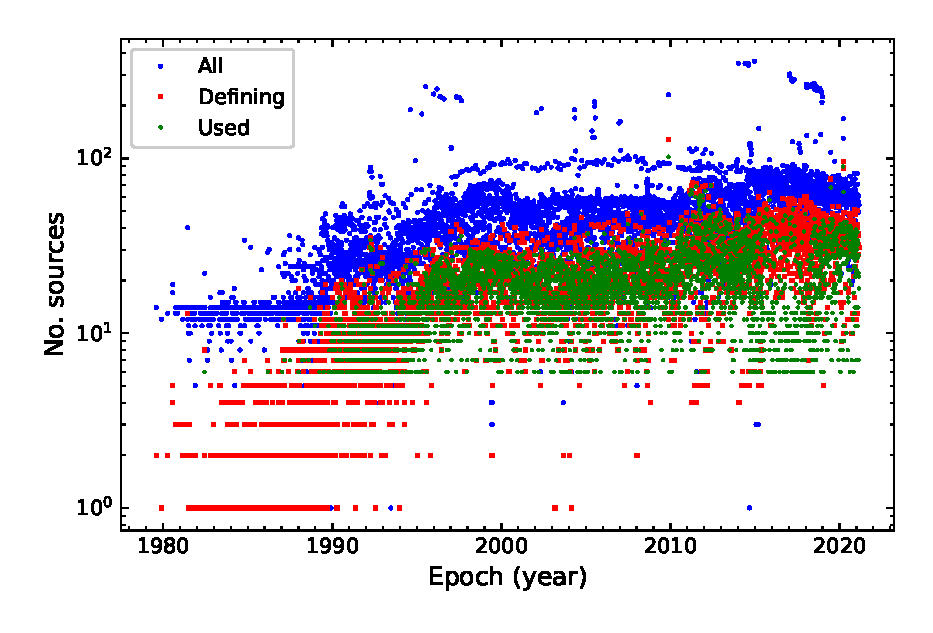
\includegraphics[width=\columnwidth]{figs/num_sou_in_sess}  %% no file extension
   \caption[]{\label{fig:waterfalls} %
	Number of sources in session-wise radio source catalogs.
	The numbers of all sources, sources among the ICRF3 defining source list, and
	sources actually used to estimate the rotation and glide are shown in different markers.
   }
 \end{figure}
% ===========================================================================
%% Have "floats" such as figures between blank lines to make them float



%% {fig:waterfalls}
%===========================================================================
 \begin{figure*}[hbtp]
   \centering
   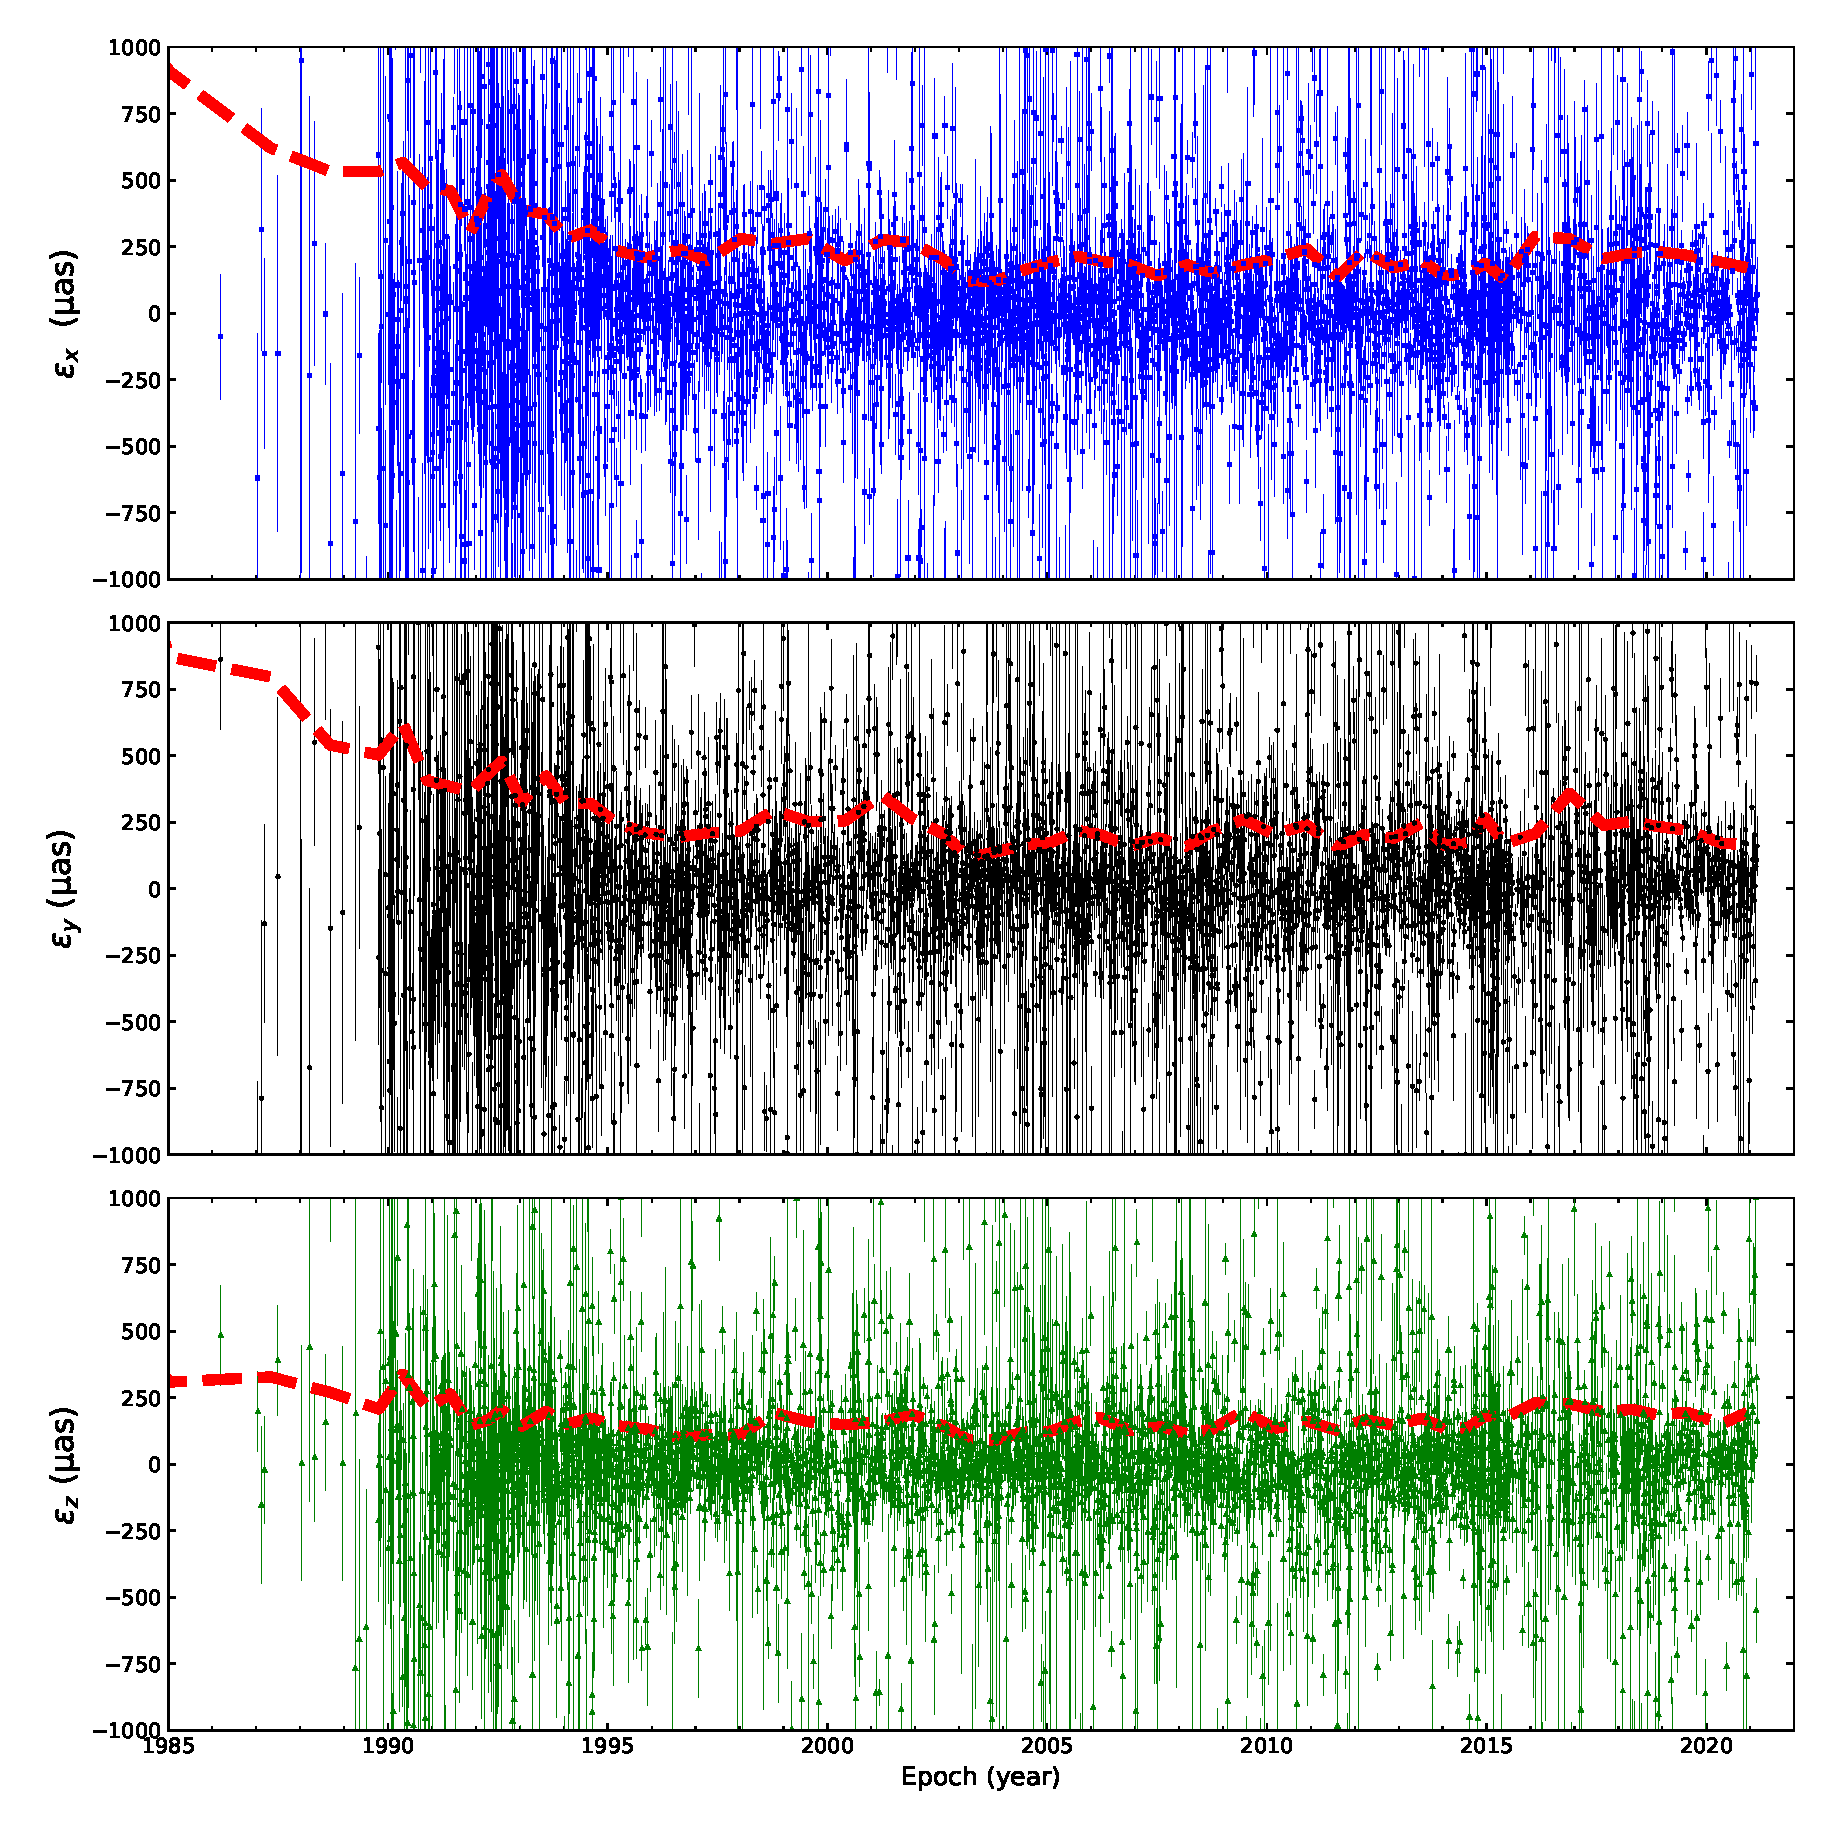
\includegraphics[width=\columnwidth]{figs/orient-from-sess-crf}  %% no file extension
   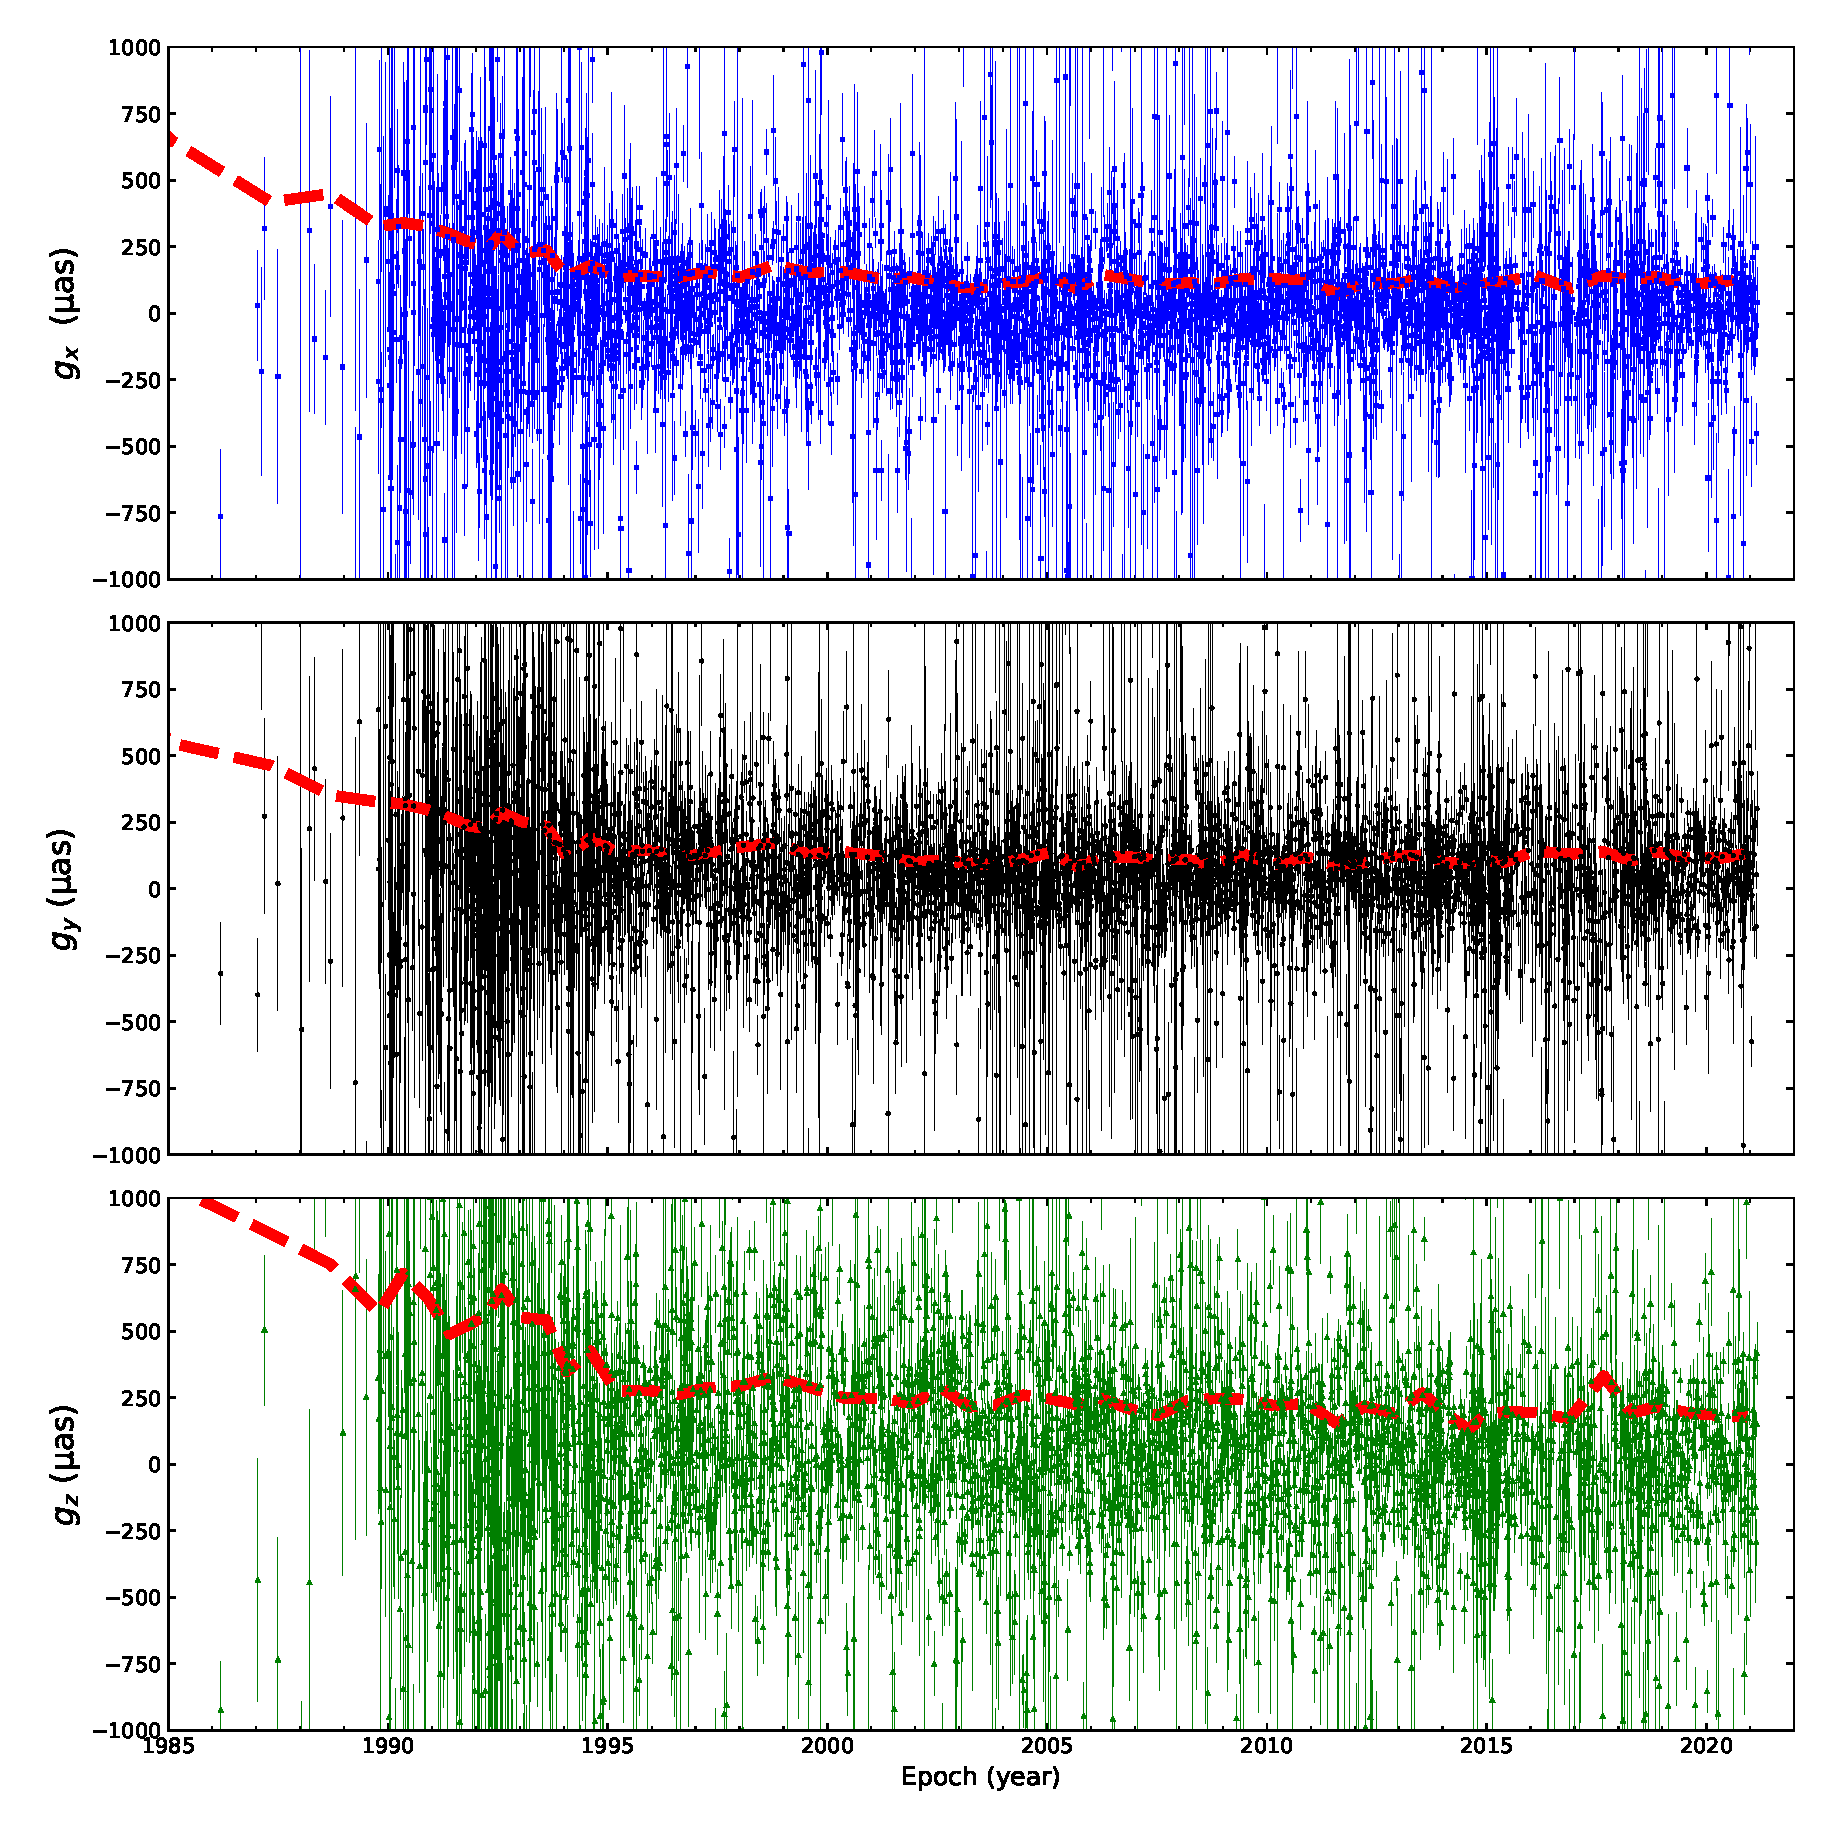
\includegraphics[width=\columnwidth]{figs/glide-from-sess-crf}  %% no file extension
   \caption[]{\label{fig:sess-wise-pmt} %
	Rotation ($left$) and glide ($right$) of session-wise CRFs with referred to
	the ICRF3 $S/X$-band catalog.
	The formal uncertainty of parameter estimate is indicated by the errorbar.
	The red dashed line shows the weighted root-mean-square (wrms) of every 100 points.
   }
 \end{figure*}
% ===========================================================================
%% Have "floats" such as figures between blank lines to make them float


%% In this file every sentence starts on a new line for better
%% readability, easier change, better synchronization in
%% shared-access systems such as svn, easier use of (mg)diff.
%% This is automatically formatted by emacs in the setup I use,
%% specified in my ~/.emacs shown in "Recipes for linux/unix"
%% on my website.


%\subsection{Method}
%%%%%%%%%%%%%%%%%%%%
% We solved the statistical equilibrium and radiative transfer equations
% for all relevant levels and frequencies in \MgI\ and \MgII\ for
% various models of the solar atmosphere, including the standard one
% formulated in the monumental articles by Vernazza et al.\
% (\citeyearads{1973ApJ...184..605V}, % VALI
% \citeyearads{1976ApJS...30....1V}, % VALII
% \citeyearads{1981ApJS...45..635V}). % VALIII
%% Example same-authors multiple citation list

%    \begin{table}
%        \centering
%        \caption{
%        Orientation offsets with referred to the ICRF3 S/X-band frame.
%        }
%        \begin{tabular}{ccccc}
%            \hline \noalign{\smallskip}
%            & $N_{\rm sou,def}$ & $R_X$ & $R_Y$ & $R_Z$  \\
%            &  &$\mathrm{\mu as}$ & $\mathrm{\mu as}$ & $\mathrm{\mu as}$  \\
%            \noalign{\smallskip}
%            \hline
%            \noalign{\smallskip}
%            ICRF2       & 296  & $ -10$  $\pm$ 7 & $ +20$  $\pm$  8 & $  -1$  $\pm$  7 \\
%            ICRF3-K     & 193  & $ -10 \pm 10$   & $ -9 \pm  11$ & $ -5$  $\pm$  7 \\
%            ICRF3-X/Ka  & 176  & $ -28$  $\pm$ 26 & $ -25$  $\pm$ 27 & $  -52$  $\pm$ 19 \\
%            \noalign{\smallskip}
%            \hline
%        % OPA2019a & 4380 & 2920 & $ +28$  $\pm$  2 & $ -50$  $\pm$  2 & $  -1$  $\pm$  1 \\
%        \end{tabular}
%    \end{table}
%
%    \begin{table}
%        \centering
%        \caption{
%        Orientation offsets with referred to the ICRF3 S/X-band frame from bootstrap sampling.
%        }
%        \begin{tabular}{cccccc}
%            \hline \noalign{\smallskip}
%            & $N_{\rm com}$ & $N_{\rm used}$ & $R_X$ & $R_Y$ & $R_Z$  \\
%            &  &  & $\mathrm{\mu as}$ & $\mathrm{\mu as}$ & $\mathrm{\mu as}$  \\
%            \noalign{\smallskip}
%            \hline
%            \noalign{\smallskip}
%            ICRF2       & 3410 & 2275 & $ -19$  $\pm$  6 & $ +22$  $\pm$  5 & $  +0$  $\pm$  4 \\
%            ICRF3-K     & 793  & 530  & $ -21$  $\pm$  8 & $ -18$  $\pm$  8 & $ -11$  $\pm$  6 \\
%            ICRF3-X/Ka  & 638  & 425  & $ -53$  $\pm$ 19 & $  -7$  $\pm$ 19 & $  +6$  $\pm$ 10 \\
%            % OPA2019a    & 4380 & 2920 & $ +28$  $\pm$  2 & $ -50$  $\pm$  2 & $  -1$  $\pm$  1 \\
%            \noalign{\smallskip}
%            \hline
%        \end{tabular}
%    \end{table}

%%%%%%%%%%%%%%%%%%%%%%%%%%%%%%%%%%%%%%%%%%%%%%%%%%%%%%%%%%%%%%%%%%%%%%%%%%%%
%\section{Conclusion} \label{sec:conclusion}
%%%%%%%%%%%%%%%%%%%%%%%%%%%%%%%%%%%%%%%%%%%%%%%%%%%%%%%%%%%%%%%%%%%%%%%%%%%%
% Our computation explained the formation of the enigmatic
% \MgI\,12\,$\mu$m emission features.
% They arise through population depletion by line photon losses and
% population replenishment from the ionic reservoir through highly
% excited levels.
% A Rydberg-channel replenishment flow is realized by
% collisionally-dominated population diffusion via ladder-wise departure
% divergence (see Fig.~\ref{fig:waterfalls} in
% Sect.~\ref{sec:computations}).
%% Note the tilde.  Fig. \ref would generate too much end-of-sentence space
%% and a line break between Fig. and the number is undesirable

%%%%%%%%%%%%%%%%%%%%%%%%%%%%%%%%%%%%%%%%%%%%%%%%%%%%%%%%%%%%%%%%%%%%%%%%%%%%
%\begin{acknowledgements}
  % We are indebted to NASA's \href{http://ui.adsabs.harvard.edu}{ADS}
  % for its magnificent literature and bibliography serving which
  % was severely missed by us -- fortunately unknowingly --
  % in pre-internet 1992.
%% us -- fortunately is A&A style; ApJ wants us---unfortunately.
%\end{acknowledgements}

%%%%%%%%%%%%%%%%%%%%%%%%%%%%%%%%%%%%%%%%%%%%%%%%%%%%%%%%%%%%%%%%%%%%%%%%%%%%
%% references
\bibliographystyle{aa-note} %% aa.bst but adding links and notes to references
%%\raggedright              %% for latex+dvips, not for pdflatex
\bibliography{example}      %% example.bib = bibtex entries copied from ADS

\end{document}
